\documentclass[brazil, a4paper,12pt]{article}
\bibliographystyle{plain}
\usepackage[brazil]{babel}
\usepackage{graphicx}
\usepackage{geometry}
\usepackage[utf8]{inputenc}
\usepackage[T1]{fontenc}
\usepackage{listings}
\usepackage{indentfirst}
\geometry{a4paper,left=3cm,right=3cm,top=2.5cm,bottom=2.93cm}

\lstset{numbers=left,
stepnumber=0,
firstnumber=1,
numberstyle=\tiny,
extendedchars=true,
breaklines=true,
frame=tb,
tabsize=2,
basicstyle=\footnotesize,
stringstyle=\ttfamily,
showstringspaces=false
}

\renewcommand{\lstlistingname}{Programa}

\begin{document}
\begin{titlepage}

  \vfill

  \begin{center}
    \begin{large}
      Universidade Federal de Ouro Preto
    \end{large}
  \end{center}

  \begin{center}
    \begin{large}
      Instituto de Ciências Exatas e Aplicadas
    \end{large}
  \end{center}

  \begin{center}
    \begin{large}
      Departamento de Computação e Sistemas
    \end{large}
  \end{center}

  \vfill

  \begin{center}
    \begin{Large}
      \textbf{LINGUAGENS DE PROGRAMAÇÃO\\[0.4cm] 
        Jogo da Velha N x N}               
    \end{Large}
  \end{center}


  \vfill

  \begin{center}
    \begin{large}
      Brenda Leite e Lima\\
      Daniel Reis
    \end{large}
  \end{center}

  \begin{center}
    \begin{large}
      Professor - Camilo Leles
    \end{large}
  \end{center}

  \vfill

  \begin{center}
    \begin{large}
      João Monlevade \\
      \today \\
    \end{large}
  \end{center}

\clearpage
\tableofcontents 
\end{titlepage}

%--------------------------------------------------------


\section{Introdução}
Este trabalho consiste no desenvolvimento de um jogo utilizando o paradigma lógico, nesse caso, a linguagem Prolog. Nesse âmbito, desenvolveu-se o tema sugerido: Jogo da Velha N x N, em que é preciso passar o N (Tamanho da matriz). Depois disso, o jogo foi feito de modo que dois usuários possam jogar, sem a opção usuário x computador. Vale ressaltar que todas tentativas de jogadas são validadas. Também, é verificado se o indivíduo ganhou com base em alguns quesitos (ter alguns desses preenchidos com 1 ou 2 - X ou O respectivamente): uma linha, coluna, diagonal principal ou diagnonal secundária. O que pode ocorrer também é dar velha, ou seja, um empate - não se consegue atingir nenhum dos 4 citados anteriormente. É de suma importância mencionar que nesse jogo, utiliza-se uma matriz que é armazenada sob a forma de lista de listas, em que guarda-se várias linhas, como no exemplo abaixo:

\begin{lstlisting}
[[0, 0, 0], [0, 0, 0], [0, 0, 0]]	    [[1, 2, 0], [1, 0, 2], [2, 0, 1]]

              1   2   3			                          1   2   3
          1 |   |   |   | 1		                    1 | X | O |   | 1
          2 |   |   |   | 2		                    2 | X |   | O | 2
          3 |   |   |   | 3		                    3 | O |   | X | 3
              1   2   3			                          1   2   3
\end{lstlisting}

Como mostrado acima, a forma de representação utilizada foi:
\begin{lstlisting}
0 -> Vazio
1 -> Jogada do Jogador 1 (X)
2 -> Jogada do Jogador 2 (O)
\end{lstlisting}

\newpage
\section{Testes de execução}

\begin{figure}[!h]
\centering
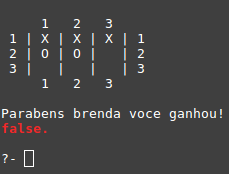
\includegraphics[width=0.5\textwidth]{img/LINHA.png}
\caption{\label{fig:fig1}Ganhando pela Linha.}
\end{figure}

\begin{figure}[!h]
\centering
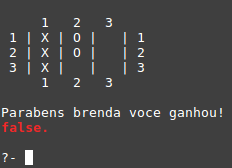
\includegraphics[width=0.5\textwidth]{img/COLUNA.png}
\caption{\label{fig:fig2}Ganhando pela Coluna.}
\end{figure}

\begin{figure}[!h]
\centering
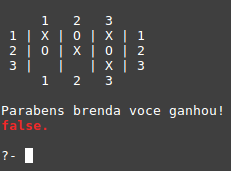
\includegraphics[width=0.5\textwidth]{img/DIAGONALPRINCIPAL.png}
\caption{\label{fig:fig3}Ganhando pela Diagonal Principal.}
\end{figure}

\newpage
\begin{figure}[!h]
\centering
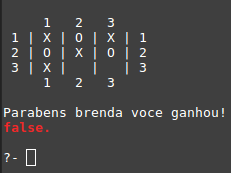
\includegraphics[width=0.5\textwidth]{img/DIAGONALSECUNDARIA.png}
\caption{\label{fig:fig4}Ganhando pela Diagonal Secundária.}
\end{figure}

\begin{figure}[!h]
\centering
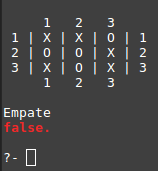
\includegraphics[width=0.33\textwidth]{img/EMPATE.png}
\caption{\label{fig:fig5}Empate.}
\end{figure}

\newpage
\section{Código em Prolog}
Nesta seção está disponibilizado o código completo do jogo.

\lstinputlisting[language=Prolog, label=cod:jogodavelha, caption={Jogo da Velha N x N usando Prolog}]{code/jogodavelha.pl}

\end{document}
